\documentclass[11pt,a4paper,twoside]{thesis}
\usepackage{graphicx}
\usepackage[utf8]{inputenc}
\usepackage[spanish]{babel}
\usepackage[left=3cm,right=3cm,bottom=3.5cm,top=3.5cm]{geometry}
\usepackage{titlesec}
\usepackage{listings}
\usepackage{xcolor}
\usepackage{hyperref}

\begin{document}

%%%% CARATULA

\def\autor{Adrian Norberto Marino}
\def\tituloTesis{Sistemas de recomendación colaborativos e híbridos}
\def\runtitulo{Resumen}
\def\runtitle{Sistemas de recomendación colaborativos e híbridos}
%\def\director{Obi-Wan Kenobi}
%\def\codirector{Master Yoda}
\def\lugar{Buenos Aires, 2022}
\newcommand{\HRule}{\rule{\linewidth}{0.2mm}}
%
\thispagestyle{empty}

\begin{center}\leavevmode

\vspace{-2cm}

\begin{tabular}{l}

\includegraphics[width=3.6cm]{logouba.png}
\end{tabular}


{\large \sc Universidad de Buenos Aires\\Facultad de Ciencias Exactas y Naturales \\ Facultad de Ingeniería}

\vspace{6.0cm}

\vspace{3.0cm}
%{
%\Large \color{red}
%\begin{tabular}{|p{2cm}cp{2cm}|}
%\hline
%& Pre-Final Version: \today &\\
%\hline
%\end{tabular}
%}
%\vspace{2.5cm}

\begin{huge}
\textbf{\tituloTesis}
\end{huge}

\vspace{2cm}

{\large Trabajo Final de Especialización en Explotación de Datos y Descubrimiento del Conocimiento}

\vspace{2cm}

{\Large \autor}

\end{center}

\vfill

{\large

%{Director: \director}

\vspace{.2cm}

%{Codirector: \codirector}

\vspace{.2cm}

\lugar
}

\newpage\thispagestyle{empty}

%
%%%% ABSTRACTS, AGRADECIMIENTOS Y DEDICATORIA
\frontmatter
\pagestyle{empty}
%\begin{center}
%\large \bf \runtitulo
%\end{center}
%\vspace{1cm}
\chapter*{\runtitulo}

\noindent Acá va un resumen del trabajo. Con el resumen se deberia poder tener una idea del trabajo en su totalidad. Desde los obetivos y los datos hasta los resultados y conclusiones. Se escibe al final. (aprox. 200 palabras).

\bigskip

\noindent\textbf{Palabras claves:} representativas del trabajo, los métodos, los datos (no menos de 5).

%\cleardoublepage
%%\begin{center}
%\large \bf \runtitle
%\end{center}
%\vspace{1cm}
\chapter*{\runtitle}

\noindent In a galaxy far, far away, a psychopathic emperor and his most trusted servant -- a former Jedi Knight known as Darth Vader -- are ruling a universe with fear. They have built a horrifying weapon known as the Death Star, a giant battle station capable of annihilating a world in less than a second. When the Death Star's master plans are captured by the fledgling Rebel Alliance, Vader starts a pursuit of the ship carrying them. A young dissident Senator, Leia Organa, is aboard the ship \& puts the plans into a maintenance robot named R2-D2. Although she is captured, the Death Star plans cannot be found, as R2 \& his companion, a tall robot named C-3PO, have escaped to the desert world of Tatooine below. Through a series of mishaps, the robots end up in the hands of a farm boy named Luke Skywalker, who lives with his Uncle Owen \& Aunt Beru. Owen \& Beru are viciously murdered by the Empire's stormtroopers who are trying to recover the plans, and Luke \& the robots meet with former Jedi Knight Obi-Wan Kenobi to try to return the plans to Leia Organa's home, Alderaan. After contracting a pilot named Han Solo \& his Wookiee companion Chewbacca, they escape an Imperial blockade. But when they reach Alderaan's coordinates, they find it destroyed - by the Death Star. They soon find themselves caught in a tractor beam \& pulled into the Death Star. Although they rescue Leia Organa from the Death Star after a series of narrow escapes, Kenobi becomes one with the Force after being killed by his former pupil - Darth Vader. They reach the Alliance's base on Yavin's fourth moon, but the Imperials are in hot pursuit with the Death Star, and plan to annihilate the Rebel base. The Rebels must quickly find a way to eliminate the Death Star before it destroys them as it did Alderaan (aprox. 200 palabras).

\bigskip

\noindent\textbf{Keywords:} War, Rebellion, Wookie, Jedi, The Force, Empire (no menos de 5). % OPCIONAL: comentar si no se quiere

%\cleardoublepage
%\chapter*{Agradecimientos}

\noindent  % OPCIONAL: comentar si no se quiere

%\cleardoublepage
%\hfill \textit{A mi persona favorita.}
  % OPCIONAL: comentar si no se quiere

%\cleardoublepage
\tableofcontents

\mainmatter
\pagestyle{headings}

%%%% ACA VA EL CONTENIDO DE LA TESIS

\chapter{Introducción}

Los sistemas de recomendación tienen por objetivo acercar a sus usuarios información productos, contenido (Textos,  audio, videos), etc..relevantes a sus preferencias o necesidades, permitiendo a estos encontrar con mayor facilidad aquello que buscan.Formalizando esta definición podemos decir que:  Los sistemas de recomendación apuntan a ayudar a un usuario o grupo de usuarios a seleccionar items de forma personalizada dado un de conjunto de items de gran extensión o un gran espacio de búsqueda.

Este objetivo puede cambiar según el contexto de cada negocio. Para un e-commerce de delivery de comidas, el objetivo es acercar a los usuarios el tipo de comida que quieren probar en ese mismo momento, a un precio que puedan pagar con tiempo de entrega aceptable. Para un e-commerce de venta de productos, se busca acercar al usuario aquellos productos que este necesitando en ese mismo momento, los cuales tienen un precio que el mismo puede pagar y por otro lado, asegurar una experiencia satisfactoria con el vendedor. En el negocio de visualización de contenido (Ya sea audio o video), el objetivo es acercar al usuario contenido a fin a sus gustos para mejorar su experiencia en la plataforma y así aumentar el engagement de sus usuarios.


Por otro lado, el objetivo de fondo siempre es el mismo, mejorar la conversión. Con esto nos referimos a aumentar el volumen de ventas para un e-commerce de venta de productos, la cantidad de deliveries mensuales, la cantidad de impresiones de publicidad  en aplicaciones de visualización de contenido, aumentar el tiempo de permanecía en las plataformas de streaming de audio o video, etc.. Podemos encontrar muchos ejemplos distintos donde el objetivo común es mejorar la conversión y engagement de los usuarios.

Desde un punto de vista mas técnico, los sistemas de recomendación se utilizan para predecir el grado de preferencia de un usuario con respecto a un item. 
En general, se puede lograr aplicando de un algoritmo de optimización, el cual minimiza la diferencia entre el grado de preferencia esperado versus real. Otros enfoques hace uso de medidas de distancia para establecer este grado de preferencia.

\section{Tipos de sistemas de recomendación}

A continuación se puede ver un gráfico que describe las clasificaciones y subclasificaciones de los sistemas de recomendación:

\begin{center}
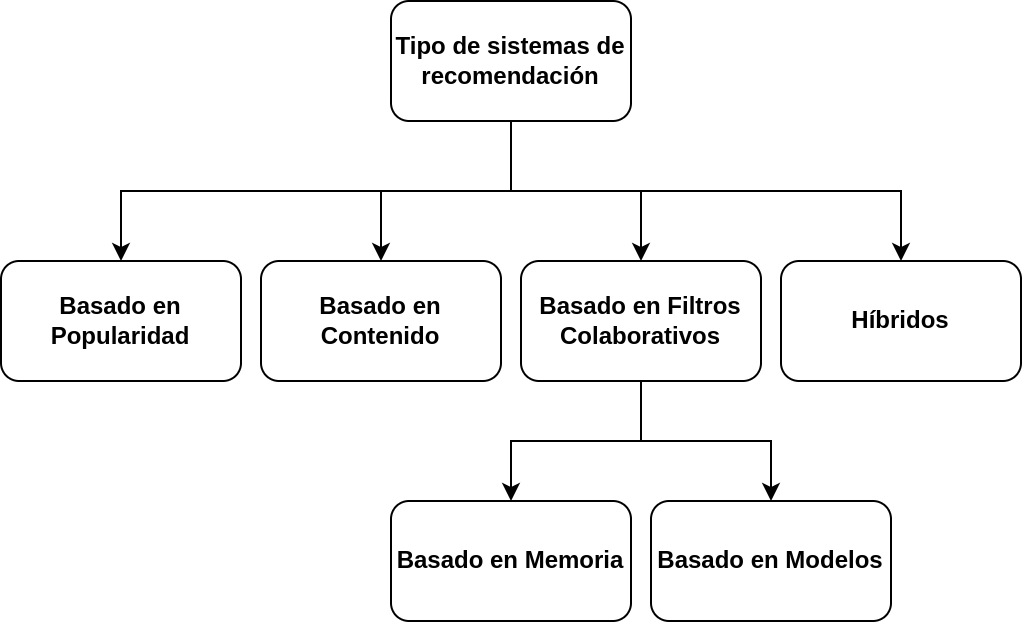
\includegraphics[width=11cm]{./images/reco-clasification.png}
\end{center}

\subsection{Basados en Popularidad} 

Este tipo de recomendador toma algunas características de popularidad de los items en cuestión, como puede ser: cantidad de vistas, cantidad de compras, cantidad de reviews positivos, etc.. Luego resuelve el top K de  los items mas populares según estos criterios. Si bien este tipo de recomendaciones tiene buenos resultandos para usuarios nuevos, de los cuales no se conocen sus preferencias, al carecer de personalización, sus recomendaciones no tienen en cuenta las preferencias de cada usuario particular, debido a que se basan en estadísticas comunes a todos los usuarios. Por esta cuestión no son considerados sistemas de recomendación per se.

\subsection{Basados en Contenido} 

A diferencia de los recomendadores basados en filtros colaborativos, este tipo de recomendador necesita un trabajo previo de ingeniería de features sobre los items, donde se busca definir que features son los mas significativos para la tarea en cuestión, y cual es el grado de adecuación de cada items con los features definidos. Por otro lado, es necesario registrar las interacciones de los usuarios. Dada estas interacciones, se puede definir el grado de preferencia de los usuarios a cada feature definido para los items. Con esta información es posible encontrar tanto items como usuarios similares y realizar recomendaciones del tipo:

\begin{itemize}
\item Dado un usuario A, el cual tiene preferencia por el item X, también podría tener preferencia por el item Y, por ser muy cercano o similar al item X.
\item Dos usuarios A y B cercanos o similares tendrán preferencias similares. De esta forma es posible recomendar item consumidos por el usuario A al usuario B y vise versa. 
\end{itemize}
	
La principal desventaja de este enfoque es que es necesario realizar ingeniería de features para encontrar los features que produzcan las mejores recomendaciones. El modelo no encuentra estos features sino que deben ser definidos de antemano. Como ventaja, si se encuentra los features correctos se pueden lograr buenos resultados.
		
\subsection{Basados en Filtrado Colaborativos} 

Estos modelos, a diferencia de los basados en contenido, no requiriere ingeniería de features, lo que los hace mas simples de implementar, ya que únicamente es necesario registrar las interacciones de los usuarios para con los items. Ejemplos interacciones podrían ser:
			\begin{itemize}
				\item El usuario A visualizo el item X el dia 2 de marzo de 2022.
				\item El usuario A compro el item X el dia 10 de marzo de 2022.
				\item El usuario A califico al item X con un 5 el dia 25 de marzo de 2022.
			\end{itemize}
			Por otro lado, estos modelos personalizan sus recomendaciones, es decir que ajustan las recomendaciones a cada usuario particular, en base a sus preferencias, al igual que los basados en contenido.
			De igual forma que los basados en contenido se puede encontrar usuario e items similares y recomendar items entre usuarios similares.

Estos modelos aprende un espacio latente de soluciones sin necesidad de recolectar datos y definir features, lo cual puede llevar a una solución sesgada. Por otro lado, no todo son rosas con estos modelos, ya que sufren un problema llamado cold start o arranque en frio. Si pensamos en una solución donde alimentamos al modelo con una ventana de interacciones de usuario-item filtrando los últimos N meses, tendremos las siguiente situaciones:

\begin{itemize}
	\item Usuarios nuevos: Los usuarios nuevos no tendrán interacciones, por lo tanto este modelo no podrá realizar ninguna recomendación. En general, se establece un mínimo de interacciones para que modelo pueda realizar recomendaciones acertadas, ya que con pocas interacciones no podrá realizar buenas recomendaciones.
	\item Usuarios con pocas interacciones: Por otro lado, tenemos a los usuarios que tienen una baja velocity en cuando a interacciones con el sistema o aplicación. Si pensamos en un e-commerce, hay usuario que compran con mucha frecuencia y otra compras muy de vez en cuando. Estos últimos en general tendrán pocas interacciones pudiendo caer por debajo del umbral mínimo que requiere el modelo. De esta forma, tendremos usuario que quedaran fuera del modelo en forma cíclica.
	\item Usuarios con muchas interacciones: Este es el caso ideal, donde el usuario tiene una gran cantidad de interacciones usuario-item. Para estos usuarios el modelo podrá ofrecer mejores recomendaciones, ya que cuanto mas interacciones se tengan, el modelo se ajusta con mas facilidad a sus preferencia.

\end{itemize}


\subsection{Híbridos}

Son aquellos modelos que combinan mas de una técnica de recomendación, también llamados ensambles de modelos.

\subsection{Tipos dentro de los basados en Filtros Colaborativos} 

Dentro de los sistemas de recomendación basados en filtros colaborativos, tenemos dos sub-clasificaciones referidas a la forma en la que se realizan las predicciones:

 \subsubsection{Basados en Memoria} 
 
 Este tipo de modelos mantiene sus datos en memoria. Se recorren todos los datos (full scan) cada vez que se necesita realizar un inferencia o predicción (fijando un número de vecinos a comparar). Un ejemplo de estos modelos es el algoritmo de k vecinos cercanos (KNN), el cual mantiene una matriz rala de distancias en memoria, la cual se recorre completamente para comparar las distancias entre filas o columnas, usando alguna medida de distancia como puede ser la distancia coseno, coseno ajustada, manhattan, etc... Para mitigar el problema de búsqueda exhaustiva se suele usar una cache para realizar las búsqueda una única vez. Otro problema es su limitación al tamaño máximo de la memoria con la que se cuente, es decir que el tamaño de la matrix depende de la memoria maxima. Esto puede mitigarse utilizando implementaciones de matrices esparsas, las cuales comprimen los datos en memoria guardando unicamente las celdas que tiene datos. Ademas, es posible utilizar un cache que mantenga en memoria las búsqueda mas frecuentes y baje a almacenamiento secundario las menos frecuentes. Todos estos problemas de performance y uso de recursos se deben a que KNN no reduce la dimensionalidad de los datos, como si lo hacen varias implementaciones basadas en embeddings, auto-encoder, redes neuronales etc.., donde lo que se buscan es encontrar una representación mas compacta de los items y usuarios sin perder información. Mas allá de tener que lidiar con esto problema de escalabilidad, los resultado obtenidos por estos modelos no están muy alejados de aquellos que se encuentra en el estado del arte. Puede recomendarse su uso cuando tenemos un dominio reducido, dada su simplicidad. 

 \subsubsection{Basados en Modelos}
 
Algunos ejemplos de estos modelos son los clasificadores bayesianos, redes neuronales, algoritmos genéticos, sistemas difusos y la técnica de descomposición matricial (SVD) en memoria. Estos modelos en general buscan directa o indirectamente reducir la dimensionalidad de los datos. De esta forma, es posible utilizarlos en dominios con una gran cantidad de datos.

\section{Descripción del problema y motivación}

Con este trabajo se busca contestar las siguientes preguntas:

\subsection{¿Los modelos basado en filtro colaborativos que utilizan técnicos de deep learning obtienen mejores resultados?}

La idea detrás de esta pregunta es realizar benchmarks sobre distintos modelos del estado de arte basados en deep learning o no, utilizando el mismo set de datos y las mismas métricas. De esta forma, se busca comprender cual es la diferencia en performance entre los modelos seleccionados. Por otro lado, se busca comprender cuando es mas adecuado utilizar cada enfoque. Como ya se comentó en el apartado de introducción, hay modelos que están mas limitados que otros según el número de recursos de hardware o interacciones con los que se cuente.

\subsection{¿Cuáles son las ventajas y desventajas de cada enfoque a la hora de aplicar estas técnicas?}

Esta pregunta se refiere a comprender cuando es conveniente aplicar una técnica u otra teniendo en cuenta las ventajas y desventajas de cada enfoque y modelo.

\subsection{¿Cómo se puede solucionar el problema de cold-start que sufre el enfoque de recomendación basado en filtros colaborativos?}

Como ya se comentó en la introducción, los modelos de filtro colaborativos necesitan un número mínimo de interacciones usuario-item para poder operar y producir recomendaciones aceptables. La propuesta es explorar enfoques que permiten lidiar con este problema. Uno de los enfoques más comunes es utilizar ensamples de modelos basados en filtros colaborativos con otros modelo basados en contenidos. Estos ensamples puede diferir en sus técnicas dependiendo del dominio de los datos.

\section{Trabajos previos ($>$ 1 carilla)}

COMPLETAR

\section{Objetivos ($>$ 1/2 carilla)}

Como primer objetivos, se pretender comprender cuales son los fundamentos teóricos sobre los que se apoya cada técnica aplicada y bajo que escenarios puede ser con conveniente aplicarlas. Por otro lado, se intenta determinar cual es la diferencia en performance de cada técnica aplicada sobre el mismo set de datos, midiendo su performance utilizando las mismas métricas. ¿Obtenemos diferencias significativas?

Como segundo objetivo se busca proponer nuevas técnicas y/o explorar técnicas existentes que permite lidiar o solucionar el problema de cold start que sufren los sistemas de recomendación basados en filtros colaborativos. Finalmente, se compararan esta técnicas mediante el benchmark propuesto para compara como se comporta cada modelos ante usuarios con escasas o ninguna interacción en el set de datos propuesto.

COMPLETAR

\chapter{Materiales y Métodos}

\section{Datos} 

Para realizar este trabajo se selecciono el dominio del cine, ya que existen conjuntos de datos bien definidor y actualizados. 
Estos datasets en general están pensados para probar modelos de recomendación. Por otro lado, es el dominio clásico en papers 
y literatura de sistemas de recomendación en general.

Dada la propuesta de este trabajo, es necesario contar con datos de interacciones de usuarios con items(películas en este caso). 
Ademas, dado que se busca solucionar el problema de cold-start para el enfoque de filtros colaborativos, se necesitara contar 
con otro enfoque de recomendación, el cual posiblemente pueda ser basado en contenido. Por esta cuestión, necesitamos contar 
con features completos y consistentes para los items(películas).

Dadas estas necesidades se decidió utilizar los siguientes datasets:


\subsection{\href{https://grouplens.org/datasets/movielens/25m/}{MovieLens 25M Dataset}}

Esta dataset prácticamente no tiene features para los items(películas) pero si tiene las calificaciones realizadas 
por los usuarios. También se cuenta con un conjunto de tags o palabras clase cargadas por los usuarios para cada 
item(película). Otro punto importante, es que todos los usuarios tienen al menos 20 interacciones, lo cual asegura
que no habrá problemas de baja performance por falta de datos. 
De esta forma, este dataset sera muy util para entrenar modelos de recomendación basados en filtros colaborativos
y ademas cuenta con columnas extras como tags, que serán útiles a la hora de entrenar modelos basados en contenido.


\subsection{\href{https://www.kaggle.com/datasets/rounakbanik/the-movies-dataset?select=movies_metadata.csv}{TMDB Movie Dataset}}


Este dataset no tiene calificaciones personalizadas de los items como si sucede con el dataset anterior, 
pero tiene varios features de los items que pueden ser muy útiles para modelos basados en contenido e inclusive
modelos híbridos, los cuales buscamos explorar.


\subsection{Preprocesamiento}

Como parte inicial se la etapa de pre-procesamiento de datos se utilizo una base de datos MongoDB. Se utilizo mongodb 
y no pandas debido a que pandas requiere cargar todo el dataset en memoria. Si bien este problema se puede lidiar 
aumentado el tamaño de la memoria swap(Linux) o la memoria virtual(windows) puede ocasionar caída de procesos y lentitudes 
innecesarias. En este caso se selecciono una base de datos de tipo document, la cual no necesita cargar todos los datos 
en memoria y por otro lado, existe la posibilidad de escalar la base de datos a mas nodos en caso de ser necesario.


Ambos dataset contiene una varios archivos csv los cuales vamos a llamar tablas, de los cuales se utilizaron los siguientes:

\begin{itemize}
	\item movie\_metadata: Pertenece al TMDB dataset. Es la fuente de verdad de donde tomamos columnas con datos de películas.
	\item tags: Pertenece al dataset MovieLens. De esta tabla se tomaron los tags o palabras clase datas de alta por los usuarios para cada película.
	\item ratings: Pertenece al dataset MovieLens. De esta tabla se tomaron las calificaciones de los usuario para las películas que fueron calificadas.
\end{itemize}

De esta forma primero se hizo un merge o join de las tabla ratings y tags por las columnas user\_id y movie\_id,
 ya que tenemos dos columnas que representan interacciones de usuarios: 

\begin{itemize}
	\item rating: Pertenece a la tabla ratings.
	\item tags: Pertenece a la tabla tags.
\end{itemize}

En segundo lugar se hizo merge entre las tablas ratings\_tags\_v1 y movie\_metadata utilizando la columnas imdb\_id, la cual es el único 
identificador único de las películas en ambas tablas.

Finalmente se termino con dos tablas como resultado:

\begin{itemize}
	\item movies\_v4.csv: Contente toda la información de las películas, incluidos todos los tags cargados por los usuarios que calificaron un película.
	\item ratings\_tags\_v1.csv: Contiene tanto las calificaciones como las tags para cada usuario y película. 
\end{itemize}

\subsubsection*{Tabla de interacciones}

La tabla ratings\_tags\_v1 tiene datos a nivel interacción usuario-item. De esta forma a nivel usuario-item se cuenta con la 
calificación de la película realizada por el usuario, ademas de los tags que el usuario cargo o ingreso para 
esa películas. Estos tags no son mas una lista de palabras que son representativas de la película en cuestión. 
Por ejemplo, para la película Toy Store deberíamos tener palabras referente a la misma como: boss, woody, 
animation, 3d, etc.. Finalmente contamos con la fecha en la cual se realizaron esta interacciones. Se entiende 
que la calificación y los tags se ingresaron en el mismo momento.


\begin{itemize}
	\item user\_id:  Existen 13.281 usuarios.
	\item movie\_id: Existen 33.444 películas.
	\item timestamp: Fecha en la cual el usuario califico el item(movie\_id). Es un string de formato año-mes. Existen valores entre 1997-09 y 2019-11 inclusive.
	\item rating:    Calificación. Es un valor discreto numérico: 0.5, 1, 1.5, 2, 2.5, 3, 3.5, 4, 4.5, 5.
	\item tags:      Lista de palabras definidas por cada usuario para una película. Se cuenta con los tags a nivel usuario-película.
\end{itemize}


\subsubsection*{Tablas de metadata de películas}

La tabla movies\_v4 cuenta con información de cada película seleccionada de ambos datasets. 

\begin{itemize}
	\item title: 	Título de la película.
	\item native\_languaje: Lenguaje original en el cual fue filmada la película.
	\item genres:  	Ambos dataset cuentan con una lista de géneros a los que adiete la película.
	\item overview:	Sinopsis de la película.
	\item poster:	Enlaces al detalle de la película en imdb y the movie database. Estos enlaces
					permiten hace join con mas datos que se encuentren en la Descripción de estos
			 		sitios pero en este trabajo solo se utilizara la imagen pata de la película
					a modo de visualización.
	\item release: 		Fecha de lanzamiento.
	\item budget: 		Presupuesto destinado para realizar el film.
	\item popularity: 	Popularidad.
	\item vote\_count: 	Cantidad de votos.
	\item vote\_mean: 	Medio de votos por película.
	\item tags:         Son los tags cargados por todos los usuario que interactuaron con la película. 
						Es la mismos información que tenemos en la tabla de interacción pero ahora a nivel item.
\end{itemize}

\subsubsection*{Valores faltantes}

Una vez generadas ambas tablas se procedió a buscar missing values. A continuación en la tabla \ref{table:tab} 
se pueden ver las columnas con missing values:
\begin{table}[h!]
\centering
\footnotesize
\begin{tabular}{lrrrrrr}
\hline
Columna &  Porcentaje de missing values \\
\hline
   	budget     &  70      \\
   	poster     &  0.00085 \\
   	release    &  0.0085  \\
	popularity &  0.00085 \\
	vote\_mean  &  4.8     \\
	vote\_count &  4.6     \\
\hline
\end{tabular}
\caption{Missing values en la tabla movies\_v4.}
\label{table:tab}
\end{table}

Luego se removieron las filas de la tabla para aquellas columnas del reporte anterior que tuvieran hasta 0.06 \% de valores faltantes. A continuación se removió la columna budget por tener un porcentaje muy alto de valores faltantes lo que la volvió inutilizable. Por otro lado, la tabla ratings\_tags\_v1 no se modifico, ya que no tenia valides faltantes en ninguna de sus columnas.


\section{Análisis exploratorio}

\chapter{Métodos ($>$ 3 carillas)}


Describir los métodos utilizados (a utilizar). 
Es obligatorio agregar un párrafo especificando a que materias se relacionan.

\section{Método I }
\section{Método II}
\section{Métricas}

\chapter{Experimentos (si los hay)}
Pueden ser comparaciones entre los métodos utilizados, por ejemplo. 

\chapter{Resultados ($>$ 3 carillas)}

Pueden ser preliminares. Es obligatorio tener algo hecho.


\chapter{Conclusiones ( $>$ 1 carilla)} 

Pueden ser preliminares. 
Si no hay mucho hecho se pueden discutir las dificultades a futuro.


%%%% BIBLIOGRAFÍA
\backmatter
%\bibliography{tesis}

\end{document}
